\pagestyle{myFancy}
\chapter{Simulation Results}
In this chapter original results from simulations are presented.
The code used to perform such simulations is based on the code originally developed for the calculations presented in refs.~\cite{Panero:2009tv,Mykkanen:2012ri}.

\section{Rotational Invariance Restoration}
This first section has the aim to reproduce the rotational invariance restoration of ref.~\cite{Lang:1982tj} for the continuous group $\SU(2)$ (and not for its discrete icosahedral subgroup $\tilde{Y}$, like explained in \secref{Sec3:RotInv}).\\
This is done by evaluating the correlator of two Polyakov loops as discussed in \secref{Sec2:PolyakovLoops}, computed on two different lattices with two different values of $\beta$, corresponding to two different lattice spacings.

\subsection{Setup of the Simulations}
The lattices are taken to be periodic in every direction, with $n_s$ sites in each spatial direction ($n_s=n_x=n_y=n_z$) and $n_t$ sites in the time direction.
The lattice has, therefore, $n_s^3n_t$ sites.\\
The simulations are run starting from a cold configuration, with $2500$ thermalization steps, where each Monte Carlo step is composed of one heat-bath step followed by three overrelaxation steps.
While the plaquette is observed to thermalize very quickly, after $O(10)$ steps in preliminary simulations with both hot and cold starts, we estimate $2500$ thermalization steps to be enough to ensure full thermalization of the configurations.\\
After thermalization, $20000$ measurements are taken of every possible independent correlator between two Polyakov loops, with $2$ updates between each measurement.\\
On a lattice with $n_s$ spatial sites in each direction, only pairs of Polyakov loops whose distance, in each spatial direction, is less than or equal to $n_s/2$ are independent: for example a pair of Polyakov loops extending for $n_s/2+1$ sites in a certain direction is equivalent to the Hermitian conjugate of a couple extending for $n_s/2-1$ sites, because of the periodic boundary conditions (see \eqref{2:nonzeroMomPolyakov}).
But, since the Polyakov loop correlator expectation value is real, they have the same numerical value.\\
\figref{4F:PolyakovPeriodic} represents a graphical visualization of this fact.
\begin{figure}[!htbp]
    \centering
    \begin{subfigure}[b]{0.48\textwidth}
        \centering
        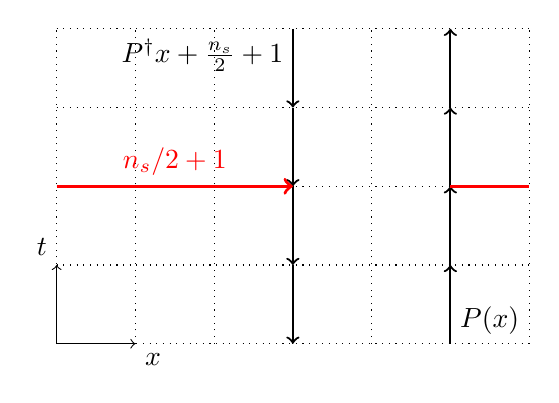
\begin{tikzpicture}
            \draw[step=1.0,dotted] (0,0) grid (6,4);
            \draw[->] (0,0) -- (1,0) node[anchor=north west]{$x$};
            \draw[->] (0,0) -- (0,1) node[anchor=south east]{$t$};
            
            \draw (5,0) node[anchor=south west]{$P(x)$};
            \draw[thick,->] (5,0) -- (5,1);
            \draw[thick,->] (5,1) -- (5,2);
            \draw[thick,->] (5,2) -- (5,3);
            \draw[thick,->] (5,3) -- (5,4);
            
            \draw (3,4) node[anchor=north east]{$P^\dagger\pr{x+\frac{n_s}{2}+1}$};
            \draw[thick,->] (3,4) -- (3,3);
            \draw[thick,->] (3,3) -- (3,2);
            \draw[thick,->] (3,2) -- (3,1);
            \draw[thick,->] (3,1) -- (3,0);
            
            \draw[very thick,red] (5,2) -- (6,2);
            \draw[very thick,red] (1.5,2) node[anchor=south]{$n_s/2+1$};
            \draw[very thick,red,->] (0,2) -- (3,2);
        \end{tikzpicture}
    \end{subfigure}
    \hfill
    \begin{subfigure}[b]{0.48\textwidth}
        \centering
        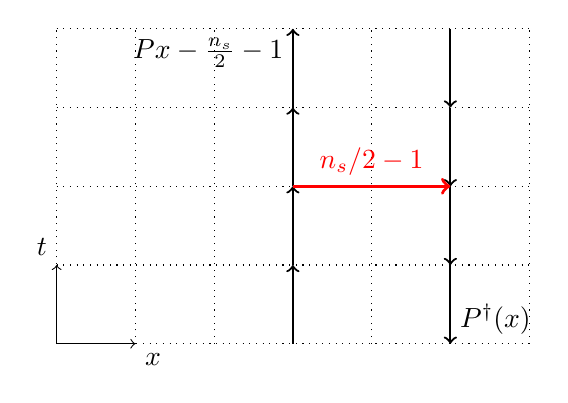
\begin{tikzpicture}
            \draw[step=1.0,dotted] (0,0) grid (6,4);
            \draw[->] (0,0) -- (1,0) node[anchor=north west]{$x$};
            \draw[->] (0,0) -- (0,1) node[anchor=south east]{$t$};
            
            \draw (5,0) node[anchor=south west]{$P^\dagger(x)$};
            \draw[thick,->] (5,4) -- (5,3);
            \draw[thick,->] (5,3) -- (5,2);
            \draw[thick,->] (5,2) -- (5,1);
            \draw[thick,->] (5,1) -- (5,0);
            
            \draw (3,4) node[anchor=north east]{$P\pr{x-\pr{\frac{n_s}{2}-1}}$};
            \draw[thick,->] (3,0) -- (3,1);
            \draw[thick,->] (3,1) -- (3,2);
            \draw[thick,->] (3,2) -- (3,3);
            \draw[thick,->] (3,3) -- (3,4);
            
            \draw[very thick,red,->] (3,2) -- (5,2);
            \draw[very thick,red] (4,2) node[anchor=south]{$n_s/2-1$};
        \end{tikzpicture}
    \end{subfigure}
    \caption{The correlator of two Polyakov loops separated by $n_s/2+1$ sites (left) is equal to the Hermitian conjugate of the correlator of two Polyakov loops at a distance of $n_s/2-1$ sites (right), \ie $\expval{P(x)P^\dagger\pr{x+\frac{n_s}{2}+1}}=\expval{P\pr{x-\pr{\frac{n_s}{2}-1}}P^\dagger(x)}^\dagger$.}
    \label{4F:PolyakovPeriodic}
\end{figure}\\
Therefore, we only consider correlators of pairs of Polyakov loops whose spatial separations are given by the lattice vectors lying within a cube of size $n_s$ having the origin $(0,0,0)$ as a vertex.
Correlators associated with the same separation vector are then averaged together, to increase statistics.
%and the uncorrelated empirical standard deviation is computed as an estimate of the error.

\subsection{Analysis of Data}
After checking that each correlator's mean value is real (the imaginary part necessarily has to be compatible with $0$ within machine precision), these averages are used to compute the potential, in units of the inverse of the lattice spacing $a$, as:
\begin{equation}
    V(x,y,z) = -\frac{1}{n_t}\ln\expval{P(0)P^\dagger(x,y,z)} \label{4:Potential}
\end{equation}
where $(x,y,z)\in\prc{(0,0,0),\dots,\pr{\frac{n_s}{2},\frac{n_s}{2},\frac{n_s}{2}}}$.
The standard deviation is computed with the usual error propagation formula.\\
Plots like \figref{3F:LangRebbi} are obtained considering a section of the lattices used, specifically the $xy$-plane, that is done by plotting only values of $V(x,y,z=0)$.\\
In order to verify that there are no anisotropies, all the three main coordinate planes are plotted in \figref{4F:PotentialPlanes}.\\
The values obtained for corresponding points in each plane are compatible with each other within their statistical uncertainties and there is no visible difference between different coordinate planes.
This justifies choosing arbitrarily one plane for each lattice.
\begin{figure}[!htbp]
    \centering
    \begin{subfigure}[t]{\textwidth}
        \centering
        \begin{subfigure}[t]{0.32\textwidth}
            \renewcommand\thesubfigure{\alph{subfigure}1}
            \includegraphics[width=\textwidth]{nt4_ns8_beta2.20/xy.png}
            \caption{$xy$-plane}
            \label{4F:PotentialPlanes48xy}
        \end{subfigure}
        \hfill
        \begin{subfigure}[t]{0.32\textwidth}
            \addtocounter{subfigure}{-1}
            \renewcommand\thesubfigure{\alph{subfigure}2}
            \includegraphics[width=\textwidth]{nt4_ns8_beta2.20/xz.png}
            \caption{$xz$-plane}
            \label{4F:PotentialPlanes48xz}
        \end{subfigure}
        \hfill
        \begin{subfigure}[t]{0.32\textwidth}
            \addtocounter{subfigure}{-1}
            \renewcommand\thesubfigure{\alph{subfigure}3}
            \includegraphics[width=\textwidth]{nt4_ns8_beta2.20/yz.png}
            \caption{$yz$-plane}
            \label{4F:PotentialPlanes48yz}
        \end{subfigure}
        \addtocounter{subfigure}{-1}
        \caption{Lattice with $n_t=4$, $n_s=8$, $\beta=2.20$.}
        \label{4F:PotentialPlanes48}
    \end{subfigure}\\
    \vspace{\baselineskip}
    \begin{subfigure}[b]{\textwidth}
        \centering
        \begin{subfigure}[b]{0.32\textwidth}
            \renewcommand\thesubfigure{\alph{subfigure}1}
            \includegraphics[width=\textwidth]{nt6_ns16_beta2.35/xy.png}
            \caption{$xy$-plane}
            \label{4F:PotentialPlanes616xy}
        \end{subfigure}
        \hfill
        \begin{subfigure}[b]{0.32\textwidth}
            \addtocounter{subfigure}{-1}
            \renewcommand\thesubfigure{\alph{subfigure}2}
            \includegraphics[width=\textwidth]{nt6_ns16_beta2.35/xz.png}
            \caption{$xz$-plane}
            \label{4F:PotentialPlanes616xz}
        \end{subfigure}
        \hfill
        \begin{subfigure}[b]{0.32\textwidth}
            \addtocounter{subfigure}{-1}
            \renewcommand\thesubfigure{\alph{subfigure}3}
            \includegraphics[width=\textwidth]{nt6_ns16_beta2.35/yz.png}
            \caption{$yz$-plane}
            \label{4F:PotentialPlanes616yz}
        \end{subfigure}
        \addtocounter{subfigure}{-1}
        \caption{Lattice with $n_t=6$, $n_s=16$, $\beta=2.35$.}
        \label{4F:PotentialPlanes616}
    \end{subfigure}
    \caption{Plots of the static quark potential in the three coordinate planes for two different lattices. The colored scale represent the potential in lattice spacing units.}
    \label{4F:PotentialPlanes}
\end{figure}
\begin{figure}[!htbp]
    \centering
    \begin{subfigure}[b]{0.48\textwidth}
        \includegraphics[width=\textwidth]{nt4_ns8_beta2.20/RotSymm.png}
        \caption{Lattice with $n_t=4$, $n_s=8$, $\beta=2.20$.}
        \label{4F:PotentialRestorationLargea}
    \end{subfigure}
    \begin{subfigure}[b]{0.48\textwidth}
        \includegraphics[width=\textwidth]{nt6_ns16_beta2.35/RotSymm.png}
        \caption{Lattice with $n_t=6$, $n_s=16$, $\beta=2.35$.}
        \label{4F:PotentialRestorationSmalla}
    \end{subfigure}
    \caption{Rotational invariance restoration of the static quark potential.}
    \label{4F:PotentialRestoration}
\end{figure}\\
In order to give a more ``complete'' view, the data from \figref{4F:PotentialPlanes48xy} and \figref{4F:PotentialPlanes616xy} are reflected relative to the $x$ and $y$ axes, obtaining the plots in \figref{4F:PotentialRestoration}.\\
In both \figref{4F:PotentialPlanes} and \figref{4F:PotentialRestoration} correlators of Polyakov loops far from the origin (the ones represented by blue dots, with values of the potential in lattice units larger than approximately $1.4$) were found to be compatible with each other.
The interesting parts of these graphics are, therefore, the dots up to the dark green shade.

\subsection{Final Remarks}
It is interesting to note the resemblance of \figref{4F:PotentialRestoration} with \figref{3F:LangRebbi}, although they are obtained in different ways and, in fact, even for different gauge groups (albeit one is a relatively dense subgroup of the other).
Note also that the values of $\beta$ we used in our simulations were slightly largr than the ones used in ref.~\cite{Lang:1982tj}, in order to have a smaller lattice spacing and to allow a finer determination of the potential.

\section{BCT Lattice}
The code used for simulations on SH lattices has been adapted to simulate $\SUN$ gauge theories on the BCT lattice.

\subsection{Formulation of the Algorithm}
The first obvious change was the number of sites: being body-centered, this lattice has twice the sites of a SH with the same sizes along the four main Euclidean axes: if the lattice has $L_\mu$ sites in the $\mu=t,x,y,z$ direction, the total number of sites is, thus, $N_{sites}=L_tL_xL_yL_z$ for a SH lattice and $N_{sites}=2L_tL_xL_yL_z$ for a BCT.

\subsubsection{Lattice Sites}
Each site has coordinates $(t,x,y,z)$ where $t = 0, 1, \dots, L_t-1$, $x = 0, 1, \dots, L_x-1$, $y = 0, 1, \dots, L_y-1$ and $z = 0, 1, \dots, L_z-1$ if the lattice is a simple hypercube.
In the original code, each site was uniquely identified by an integer $0 \leq s < N_{sites}$ obtained through the following computation:
\begin{equation}
    s = z + L_z\pr{y + L_y\pr{x + L_xt}} \label{4:siteIndexSH}
\end{equation}
and the coordinates could be obtained as:
\begin{align*}
    z =& s \mod L_z \\
    y =& \frac{s - z}{L_z} \mod L_y \\
    x =& \pr{\pr{\frac{s - z}{L_z} - y}/L_y} \mod L_x \\
    t =& \pr{\pr{\frac{s - z}{L_z} - y}/L_y - x}/L_x \numthis\label{4:siteIndexSHinverted}
\end{align*}
On a BCT lattice, each site has either all integer or all half-integer coordinates.\\
If they are all integer, $s$ is computed as:
\begin{equation}
    s = 2\pr{z + L_z\pr{y + L_y\pr{x + L_xt}}} \label{4:siteIndexBCTeven}
\end{equation}
Otherwise, it is computed as:
\begin{equation}
    s = 1 + 2\pr{\prs{z} + L_z\pr{\prs{y} + L_y\pr{\prs{x} + L_x\prs{t}}}} \label{4:siteIndexBCTodd}
\end{equation}
where $\prs{x}$ represents the \emph{integer part} of $x$.\\
The inverse relation is the same as \eqref{4:siteIndexSHinverted}, but with $s$ replaced with $s/2$ if $s$ is even, otherwise, if $s$ is odd, it becomes:
\begin{align*}
    z =& \pr{\frac{s-1}{2} \mod L_z} + \frac12 \\
    y =& \pr{\frac{\frac{s-1}{2} - \prs{z}}{L_z} \mod L_y} + \frac12 \\
    x =& \pr{\pr{\pr{\frac{\frac{s-1}{2} - \prs{z}}{L_z} - \prs{y}}/L_y} \mod L_x} + \frac12 \\
    t =& \pr{\pr{\pr{\frac{\frac{s-1}{2} - \prs{z}}{L_z} - \prs{y}}/L_y - \prs{x}}/L_x} + \frac12 \numthis\label{4:siteIndexBCToddInverted}
\end{align*}
In the code, the integer $s$ is stored in the variable \texttt{site} and the coordinates $t$, $x$, $y$, $z$ are always stored in integer variables as their integer part.
An additional variable \texttt{halfInt}, that can only take values $0$ or $1$, is used to keep track whether the coordinates are integer or half-integer.

\subsubsection{Directions}
Another important part of the implementation of the lattice geometry in the code is how the different possible directions are referred to.
Each site in the SH lattice has only $8$ nearest neighbours, identified by $4$ different directions, the vectors $\pr{1,0,0,0}$ (direction $0$), $\pr{0,1,0,0}$ (direction $1$), $\pr{0,0,1,0}$ (direction $2$), $\pr{0,0,0,1}$ (direction $3$), and their opposites.\\
In the original version of the code, two arrays of dimension $4N_{sites}$, \texttt{neighbour\_plus} and \texttt{neighbour\_minus}, were used to store each site's nearest neighbours.\\
As explained in \secref{Sec3:BCT}, each site of the BCT lattice, instead, has $24$ nearest neighbours, in $12$ different directions.
The two arrays are therefore changed to size $12N_{sites}$, with the following index convention:
\begin{table}[!htbp]
    \centering
    \begin{tabular}{ |c|c|c| }
        \hline
        Direction & \texttt{dir\_plus}  & \texttt{dir\_minus}  \\\hline\hline
        0  & $\pr{  +1,   0,   0,   0}$ & $\pr{  -1,   0,   0,   0}$ \\\hline
        1  & $\pr{   0,  +1,   0,   0}$ & $\pr{   0,  -1,   0,   0}$ \\\hline
        2  & $\pr{   0,   0,  +1,   0}$ & $\pr{   0,   0,  -1,   0}$ \\\hline
        3  & $\pr{   0,   0,   0,  +1}$ & $\pr{   0,   0,   0,  -1}$ \\\hline
        4  & $\pr{+1/2,+1/2,+1/2,+1/2}$ & $\pr{-1/2,-1/2,-1/2,-1/2}$ \\\hline
        5  & $\pr{+1/2,+1/2,+1/2,-1/2}$ & $\pr{-1/2,-1/2,-1/2,+1/2}$ \\\hline
        6  & $\pr{+1/2,+1/2,-1/2,+1/2}$ & $\pr{-1/2,-1/2,+1/2,-1/2}$ \\\hline
        7  & $\pr{+1/2,-1/2,+1/2,+1/2}$ & $\pr{-1/2,+1/2,-1/2,-1/2}$ \\\hline
        8  & $\pr{-1/2,+1/2,+1/2,+1/2}$ & $\pr{+1/2,-1/2,-1/2,-1/2}$ \\\hline
        9  & $\pr{+1/2,+1/2,-1/2,-1/2}$ & $\pr{-1/2,-1/2,+1/2,+1/2}$ \\\hline
        10 & $\pr{+1/2,-1/2,-1/2,+1/2}$ & $\pr{-1/2,+1/2,+1/2,-1/2}$ \\\hline
        11 & $\pr{+1/2,-1/2,+1/2,-1/2}$ & $\pr{-1/2,+1/2,-1/2,+1/2}$ \\\hline
    \end{tabular}
    \caption{Directions index convention for the BCT lattice.}
    \label{4T:DirsBCT}
\end{table}\\
This is done in the initialization routine, in file \coderef{A1:initialize117}{initialize.cc}, from line \texttt{117} to line \texttt{672}.
In the \texttt{neighbour\_plus} array nearest neighbours in \emph{positive} directions for each site are saved, where sites are represented stored in the integer variable \texttt{next\_site} explained in \eqref{4:siteIndexBCTeven} and \eqref{4:siteIndexBCTodd}.
In the \texttt{neighbour\_minus} array nearest neighbours in \emph{negative} directions for each site are saved.

\subsubsection{Staples}
The central part of the algorithm is the computation of the staples.
As explained in \secref{Sec3:BCTlatticeGaugeTheories}, using action \eqref{3:BCTAction}, the plaquettes are triangular, therefore the staples are computed in a different way than in the case of the SH lattice.\\
For this reason, an array, called \texttt{stapleDirs}, is used to keep track of all possible staples that can be formed for any of the $12$ possible directions (this was not necessary in the SH case as staples were easier to be computed, since there were far less possible directions).
In lines \texttt{743} to \texttt{1063} of \coderef{A1:initialize743}{initialize.cc} this array is initialized in the following way: for each direction, $4$ pairs of directions are given.
A plus sign indicates a direction from the \texttt{dir\_plus} coloumn of \tabref{4T:DirsBCT}, while a minus sign indicates a direction from the \texttt{dir\_minus} coloumn of the same table.
Direction $0$ is labelled as $24$ in order to ensure that $\pr{+1,0,0,0}$ and $\pr{-1,0,0,0}$ are treated as distinct (whereas that would not be the case, if it was denoted by $0$, since $+0=-0$).\\
Each of the four pairs is such that the vector sum of the two directions forming the staple is equal to the vector representing the direction on which the considered link is defined.
For example, in line \texttt{746}, the first staple of \texttt{dir}$=0$, that is represented by $\pr{+1,0,0,0}$, is formed by directions $+4$ and $-8$, which correspond respectively to vectors $\pr{+1/2,+1/2,+1/2,+1/2}$ and $\pr{+1/2,-1/2,-1/2,-1/2}$.
As can be easily checked, $\pr{+1/2,+1/2,+1/2,+1/2}+\pr{+1/2,-1/2,-1/2,-1/2}=\pr{+1,0,0,0}$.\\
In \secref{Sec3:BCTlatticeGaugeTheories} it is stated that ``each edge is shared between eight triangles'', meaning that for each direction there must be eight different staples.
The four remaining ones are obtained from the ones already written, the \emph{positive} staples, by exchanging the first direction of each pair with the second and will be referred to as \emph{negative} staples\footnote{This is a reminiscence of the original version of the code, where \emph{positive} and \emph{negative} staples were not independent from each other, therefore were computed in two different routines in order to avoid over-counting when evaluating the plaquettes. This is not necessary anymore on the BCT lattice, as \emph{positive} and \emph{negative} staples are not counted twice.}.\\
In \figref{4F:Staples} a visual representation of this process is shown.
\begin{figure}[!htbp]
    \centering
    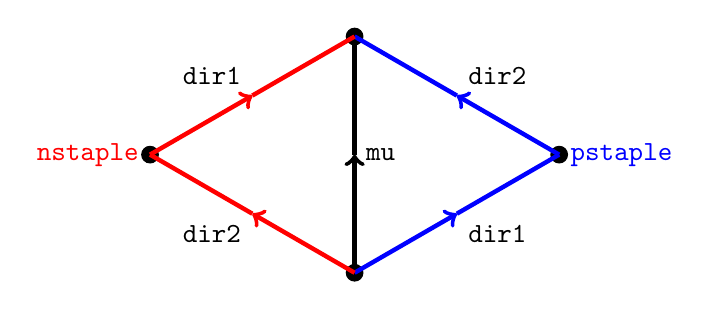
\begin{tikzpicture}
        \filldraw[black]  (0,0) circle (3pt);
        \filldraw[black]  (0,3) circle (3pt);
        \filldraw[black]  (2.598,1.5) circle (3pt);
        \filldraw[black]  (-2.598,1.5) circle (3pt);
        \draw[ultra thick,->] (0,0) -- (0,1.5) node[anchor=west]{\texttt{mu}};
        \draw[ultra thick   ] (0,1.5) -- (0,3);
        
        \draw[blue, ultra thick,->] (0,0) -- (2.598/2,1.5/2) node[text=black, anchor=north west]{\texttt{dir1}};
        \draw[blue, ultra thick   ] (2.598/2,1.5/2) -- (2.598,1.5) node[anchor=west]{\texttt{pstaple}};
        \draw[blue, ultra thick,->] (2.598,1.5) -- (2.598/2,1.5+1.5/2) node[text=black, anchor=south west]{\texttt{dir2}};
        \draw[blue, ultra thick   ] (2.598/2,1.5+1.5/2) -- (0,3);
        
        \draw[red, ultra thick,->] (0,0) -- (-2.598/2,1.5/2) node[text=black, anchor=north east]{\texttt{dir2}};
        \draw[red, ultra thick   ] (-2.598/2,1.5/2) -- (-2.598,1.5) node[anchor=east]{\texttt{nstaple}};
        \draw[red, ultra thick,->] (-2.598,1.5) -- (-2.598/2,1.5+1.5/2) node[text=black, anchor=south east]{\texttt{dir1}};
        \draw[red, ultra thick   ] (-2.598/2,1.5+1.5/2) -- (0,3);
    \end{tikzpicture}
    \caption{Representation of a \emph{positive} staple (\textcolor{blue}{\texttt{pstaple}}) and a \emph{negative} staple (\textcolor{red}{\texttt{nstaple}}). \texttt{dir1} and \texttt{dir2} represent the two directions forming the staple and \texttt{mu} represent the direction on which is defined the link variable considered.}
    \label{4F:Staples}
\end{figure}\\
Staples are then evaluated by dedicated routines, \coderef{A1:pstaple}{f4pstaple.cc} and \coderef{A1:nstaple}{f4nstaple.cc} for \emph{positive} and \emph{negative} staples respectively.
Their value is used each time the algorithm performs a heat bath or an overrelaxation step, as illustrated in \secref{Sec2:MonteCarlo}, and each time the plaquette needs to be evaluated.

\subsubsection{Plaquette}
In the original version of the code, plaquettes were evaluated by a dedicated routine, \coderef{A1:plaquette}{plaquette.cc}, that summed over all possible plaquettes and, after taking the real part of its trace, divided by a normalization factor (in order to compute the mean value).\\
The normalization factor is the total number of possible plaquettes, obtained as $D(D-1)N_{sites}$, where $D$, the number of spacetime dimensions, is the number of possible ways of choosing the ``first'' direction $\mu$ and $D-1$ is the number of possible ways of choosing the ``second'' direction $\nu$.
This is done in line \texttt{71} of \coderef{A1:plaquette}{plaquette.cc}.
In the code's normalization factor appears also \texttt{Ncol} that is needed to ensure proper normalization of the trace.\\
For the BCT lattice the code is not very different, as the principle is the same: the number of sites and of directions were changed to the ones of the BCT lattice, the staples were computed with the dedicated routines described earlier, and the normalization factor was changed to \texttt{nStaples} times \texttt{nlinks}, where \texttt{nStaples} is the number of plaquettes for each link and \texttt{nlinks} is the total number of links in the considered lattice.

\subsection{Numerical Results}
This code has been used to perform simulations of $\SU(2)$ gauge theories, in particular the mean value of the triangular plaquette (the real part of the trace of \eqref{3:PlaqTriang}) has been studied.

\subsubsection{Plaquette Mean Value as a Function of Computer Time}
Simulations have been run starting from cold configurations: $2000$ measurements have been taken for four different values of $\beta=1,2,4,8$, without thermalization, in order to study the convergence of the plaquette's average value.\\
The simulations were run on two different lattices and one update, composed of one heat bath step followed by thrree overrelaxation steps, was made between each measurement.\\
Results are shown in \figref{4F:PlaqIterBCT}.
\begin{figure}[!htbp]
    \centering
    \begin{subfigure}[b]{0.49\textwidth}
        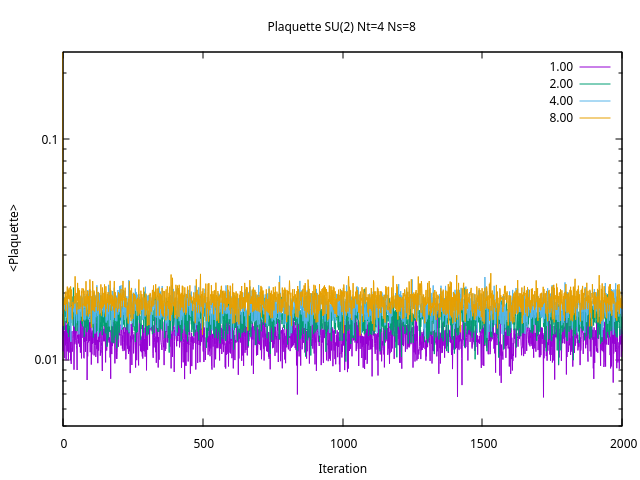
\includegraphics[width=\textwidth]{plaquetteSmallBCT.png}
        \caption{Lattice with $n_t=4$, $n_s=8$.}
        \label{4F:PlaqIterSmallBCT}
    \end{subfigure}
    \begin{subfigure}[b]{0.49\textwidth}
        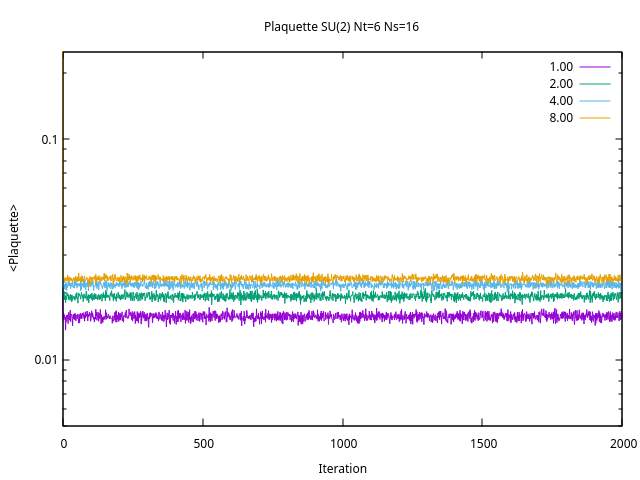
\includegraphics[width=\textwidth]{plaquetteBigBCT.png}
        \caption{Lattice with $n_t=6$, $n_s=16$.}
        \label{4F:PlaqIterBigBCT}
    \end{subfigure}
    \caption{Average value of the triangular plaquette on BCT lattices as a function of the number of iterations. The different colors represent different values of $\beta$.}
    \label{4F:PlaqIterBCT}
\end{figure}\\
In both figures it is clear that the plaquette thermalizes very quickly (only the first few values are significantly different from the others); this is expected, since, like on the hypercubic lattice, the plaquette is a very local quantity, which can be efficiently sampled by the local updates used in the code.
One can also observe that the results from the lattice with most sites have the smallest statistical fluctuations: an effect due to volume averaging.\\
The same simulation has been run on a SH lattice, computing the mean value of the rectangular plaquette \eqref{2:LatticePlaquette}, in order to make a comparison.\\
Results are shown in \figref{4F:PlaqIterSH}.
\begin{figure}[!htbp]
    \centering
    \begin{subfigure}[b]{0.49\textwidth}
        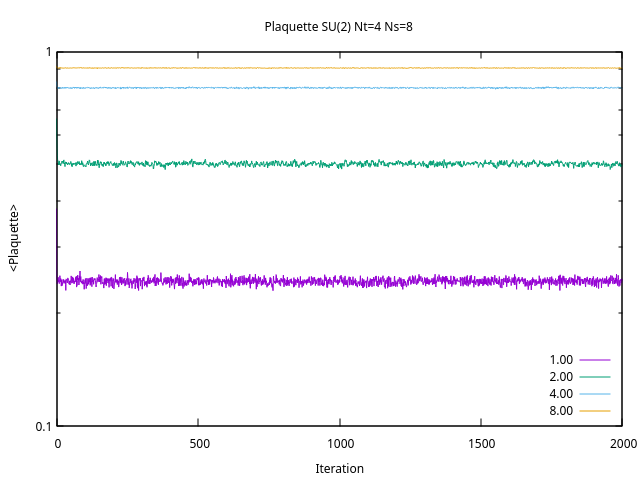
\includegraphics[width=\textwidth]{plaquetteSmallSH.png}
        \caption{Lattice with $n_t=4$, $n_s=8$.}
        \label{4F:PlaqIterSmallSH}
    \end{subfigure}
    \begin{subfigure}[b]{0.49\textwidth}
        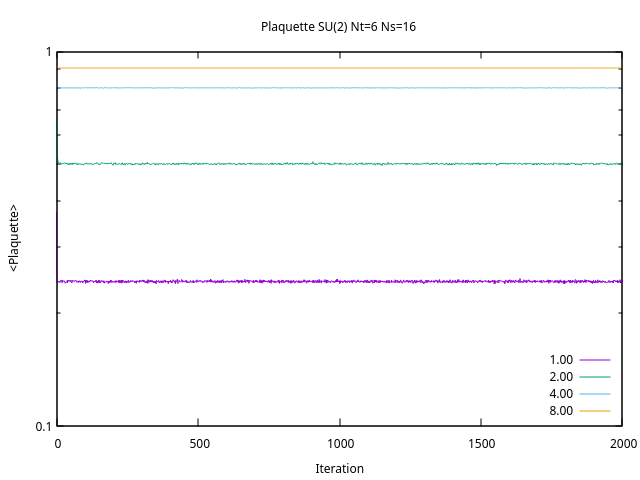
\includegraphics[width=\textwidth]{plaquetteBigSH.png}
        \caption{Lattice with $n_t=6$, $n_s=16$.}
        \label{4F:PlaqIterBigSH}
    \end{subfigure}
    \caption{Average value of the rectangular plaquette on SH lattices as a function of the number of iterations. The different colors represent different values of $\beta$.}
    \label{4F:PlaqIterSH}
\end{figure}\\
Here it can be seen that mean values of the plaquette are more distant from each other than in the BCT case.
They also have smaller fluctuations, albeit the fact that they get smaller by increasing the number of sites of the lattice is observed in both the SH and BCT cases.

\subsubsection{Plaquette Mean Value vs $\beta$}
The mean value of each dataset of \figref{4F:PlaqIterBCT} has also been computed, with the aim of studying the behaviour of the average plaquette with respect to $\beta$.
In the computation of the means, only the last $1000$ values have been taken into account, in order to discard unthermalized values.
\begin{figure}[!htbp]
    \centering
    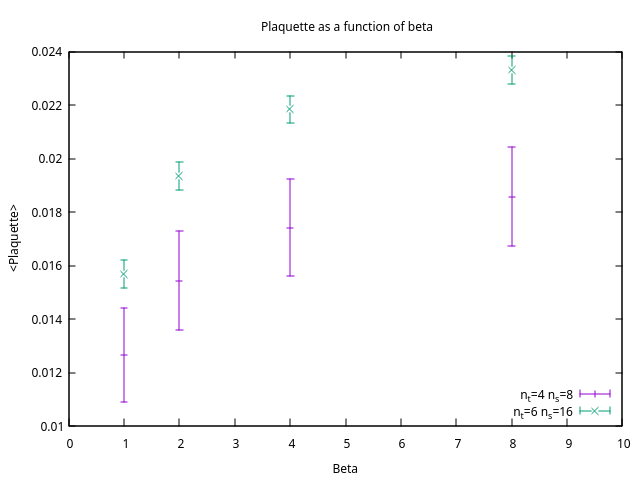
\includegraphics[width=0.5\textwidth]{PlaquetteBetaBCT.png}
    \caption{Mean value of the triangular plaquette on BCT lattices as a function of $\beta$. The purple data is from the smaller lattice ($n_t=4$, $n_s=8$), the green one is from the bigger lattice ($n_t=6$, $n_s=16$).}
    \label{4F:PlaqBetaBCT}
\end{figure}\\
As anticipated, statistical fluctuations of the lattice with a larger number of sites are smaller, thus the statistical uncertainties are smaller than error bars of points obtained from datasets of the lattice with fewer points.\\
\figref{4F:PlaqBetaBCT} reveals that, for these simulations, the plaquette mean values from lattices of different size are not compatible with each other for the same value of $\beta$, and that the dependence on $\beta$ appears not to be compatible with continuum-scaling behavior yet. For this reason, the data cannot be directly compared with \figref{3F:AvgPlaqBCTSH}, which was independently obtained with a different algorithm (and including some different normalizations, too). In fact, it is worth emphasizing that (assuming that there are no bugs in the code) it is only in the continuum limit that the results obtained from different lattice simulations should converge to the same limit.\\
As a side remark, one should also consider that, while the Monte~Carlo history of the average plaquette does not reveal exceedingly long autocorrelation times, some autocorrelation may still be present in the sample of configurations used for this preliminary analysis; in order to study this possibility in a more systematic way, one should carry out a careful analysis of other observables, too -- including, in particular, those that are of non-local nature, since typically they are most severely affected by autocorrelation problems. A typical example could be the topological charge, which (in simulations on standard hypercubic lattices) is notorious for its dramatically long autocorrelation times on fine lattices~\cite{Schaefer:2010hu}. While a systematic study of this quantity could potentially yield further motivation to carry out simulations on a BCT lattice (where better recovery of rotational symmetry can be achieved at coarser lattice spacings), this is clearly beyond the scope of the present M.Sc. thesis work, and we leave it for a dedicated future project~\cite{Aliberti:2024soa}.
%Although the first problem could be ``circumvented'' by considering the autocorrelation of the data, thus increasing the error bars, the second one has not a simple explanation and leads to think that there could be a possible bug in the code.\\
%Again, in order to make a comparison, the same plot has been reproduced for the SH lattice, using the last $1000$ data from each dataset of \figref{4F:PlaqIterBCT}.\\
%Results are shown in \figref{4F:PlaqBetaSH}.
%\begin{figure}[!htbp]
%    \centering
%    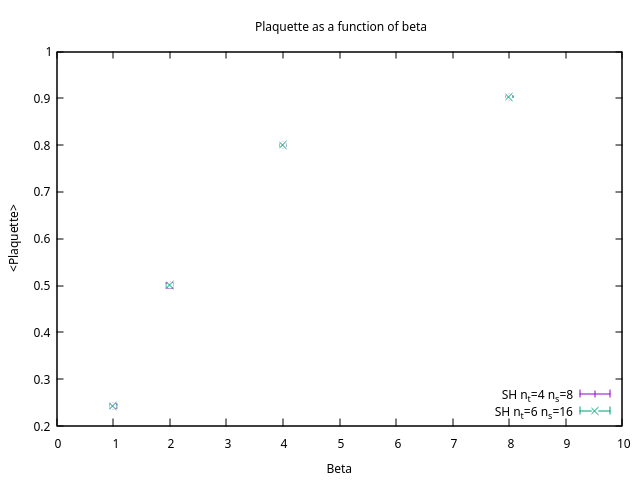
\includegraphics[width=0.5\textwidth]{PlaquetteBetaSH.png}
%    \caption{Mean value of the rectangular plaquette on SH lattices as a function of $\beta$. The purple data is from the smaller lattice ($n_t=4$, $n_s=8$), the green one is from the bigger lattice ($n_t=6$, $n_s=16$).}
%    \label{4F:PlaqBetaSH}
%\end{figure}
%This plot makes even more evident the problems mentioned before: in SH lattices, error bars are orders of magnitude smaller than those of BCT lattices and the average value of the plaquettes does not evidently depend on the size of the lattice.
%Furthermore, increasing $\beta$ (therefore decreasing the coupling constant $g$, \ie weakening the interaction) makes the averages tend to $1$, much more than the data obtained from BCT lattices and a lot more in accordance with \figref{3F:AvgPlaqBCTSH}.\\
%This is probably due to an error in the code, that needs to be investigated further.
